\documentclass[10pt,a4j]{article}
%\usepackage{graphicx,wrapfig}
\usepackage{graphicx}
\usepackage{showkeys}
\setlength{\topmargin}{-1.5cm}
%\setlength{\textwidth}{16.5cm}
%\setlength{\textwidth}{14.5cm}
\setlength{\textheight}{25.2cm}
\newlength{\minitwocolumn}
\setlength{\minitwocolumn}{0.5\textwidth}
\addtolength{\minitwocolumn}{-\columnsep}
%\addtolength{\baselineskip}{-0.1\baselineskip}
%
\def\Mmaru#1{{\ooalign{\hfil#1\/\hfil\crcr
\raise.167ex\hbox{\mathhexbox 20D}}}}
%
\begin{document}
\newcommand{\fat}[1]{\mbox{\boldmath $#1$}}
\newcommand{\D}{\partial}
\newcommand{\w}{\omega}
\newcommand{\ga}{\alpha}
\newcommand{\gb}{\beta}
\newcommand{\gx}{\xi}
\newcommand{\gz}{\zeta}
\newcommand{\vhat}[1]{\hat{\fat{#1}}}
\newcommand{\spc}{\vspace{0.7\baselineskip}}
\newcommand{\halfspc}{\vspace{0.3\baselineskip}}
\bibliographystyle{unsrt}
\newcommand{\twofig}[2]
 {
   \begin{figure}
     \begin{minipage}[t]{\minitwocolumn}
         \begin{center}   #1
         \end{center}
     \end{minipage}
         \hspace{\columnsep}
     \begin{minipage}[t]{\minitwocolumn}
         \begin{center} #2
         \end{center}
     \end{minipage}
   \end{figure}
 }
%%%%%%%%%%%%%%%%%%%%%%%%%%%%%%%%%
%\vspace*{\baselineskip}
\begin{flushright}
	Civil Engineering I\\
	April 23, 2020
\end{flushright}
\begin{center}
	{\Large \bf Lecture Note 1}
\end{center}
%%%%%%%%%%%%%%%%%%%%%%%%%%%%%%%%%%%%%%%%%%%%%%%%%%%%%%%%%%%%%%%%
\section{Review of Vector Algebra}
\subsection{Scalar and vector quantites}
A scalar is a quantity that has only a magnitude, while a vector has both magnitude(or length) and direction. The examples of frequently used scalar quantities in physics and engineering are mass, temperature, concentration, length, weight, and so on. It is sometimes useful to denote vectors by arrows typically when the geometrical relationship among vectors is of interest. In that situation, the length and orientation of the arrow indicate the magnitude and direction of the vector, respectively (see Fig.\ref{fig:fig1}). However, symbolic representations of vectors are more manipulative and convenient for rigorous discussion. 
\begin{figure}[h]
	\begin{center}
	\includegraphics[width=0.2\linewidth]{arrow.eps} 
	\end{center}
	\caption{A vector $\fat{a}$ shown graphically by an arrow.} 
	\label{fig:fig1}
\end{figure}
\subsection{Vector Identity}
Two vectors $\fat{a}$ and $\fat{b}$ are considered identical 
if their magnitude and direction are equal. In that case, we write $\fat{a}=\fat{b}$ regardless of their locations (see, Fig.\ref{fig:fig2}-(a)). For example, when two forces ($\fat{f}, \fat{g}$) of equal magnitude and direction are acting at two different locations on a body, $\fat{f}$ and $\fat{g}$ are considered mathematically identical although they are physically different forces (Fig.\ref{fig:fig2}-(b)). The exception of this rule is position vectors. The origin of position vectors are always taken at the origin of a predefined coordinate as illustrated in Fig.\ref{fig:fig2}-(c). The position vectors should be defined in this way since the correspondence between spatial points and position vectors must be one-to-one. 
\begin{figure}[h]
    \begin{center}
    \includegraphics[width=0.7\linewidth]{identity.eps} 
    \end{center}
    \caption{(a),(b)Pairs of mathematically identical vectors. 
    (c) An illustration of position vectors.} 
    \label{fig:fig2}
\end{figure}
\subsection{Basic algebraic operation on vectors}
The most fundamental algebraic operations on vectors are (1)scalar mutiplication and (2)vector addition, which are introduced as follows.
\subsubsection{Scalar multiplication}
A multiplication between a scalar $s$ and a vector $a$ is called "scalar multiplication", and is written as $s\fat{a}$. For $s>0$, scalar multiplication $s\fat{a}$ strecthes (compresses) $\fat{a}$ 
by $s$ times if $s \geq 1 (s<1)$ without changing the direction(see Fig.\ref{fig:fig3}-(a) and (b)).
When $s<0$, the scalar multiplication first reverses the directoin and then stretches or compresses 
$\fat{a}$ by $|s|$ times (see Fig.\ref{fig:fig3}-(c) and (d)).
The followings are obvious consequences of the definition of scalar multiplication. 
\begin{itemize}
\item 
    $1\fat{a}=\fat{a}$,
\item 
    $0\fat{a}=\fat{0}$,
\item
    (st)\fat{a}=s(t\fat{a}),
\end{itemize}
where $s$ and $t$ are arbitrary scalars, and $\fat{0}$ means the vector of zero length.
For $s=-1$, we write the scalar multiplication $-1\fat{a}$ simply as $-\fat{a}$.
\begin{figure}[h]
    \begin{center}
    \includegraphics[width=0.7\linewidth]{smul.eps} 
    \end{center}
    \caption{The results of scalar multiplications $s\fat{a}$ dependent on the scalar $s$.} 
    \label{fig:fig3}
\end{figure}
\subsubsection{Vector addition}
Vector addition is an operation that produces a new vector 
by connecting a pair of vectors. If we let $\fat{a}$ and $\fat{b}$ be two arbitrary vectors, we can form a directed broken line by connecting the tail of one vector with the head of the other. The sum $\fat{a}+\fat{b}$ is defined to be a vector extending from the origin of the broken line to its head. The followings are the direct onsenqueces of this definition.
\begin{equation}
    \fat{a}+\fat{0} = \fat{0}+\fat{a}=\fat{a}. 
    \label{eqn:add_zero_vec}
\end{equation}
\begin{equation}
    \left(s+t \right)\fat{a}= s\fat{a}+ t\fat{a}
    \label{eqn:dist_scalar}
\end{equation}
\begin{equation}
    s(\fat{a}+\fat{b})=s\fat{a}+s\fat{b}
    \label{eqn:dist_vec}
\end{equation}
Note that vector addition is "commutative" because Fig.\ref{fig:fig4}-(a) is showing that
\begin{equation}
    \fat{a}+\fat{b}=\fat{b}+\fat{a}
    \label{eqn:cmmt_vec_add}
\end{equation}
always holds true. This means the order of summation can be exchanged. We can add more than two vectors by repeating the pairwise vectors addition. For example, we may add three vectors either by 
\[
    \fat{a}+\left( \fat{b}+\fat{c} \right),
\]
or by 
\[
    \left( \fat{a}+\fat{b} \right) + \fat{c}.
\]
We can prove graphically that the additions above result in a same vector. Hence,
\begin{equation}
    \fat{a}+\left( \fat{b}+\fat{c} \right)
    =
    \left( \fat{a}+\fat{b} \right) + \fat{c}.
    \label{eqn:assct_vadd}
\end{equation}
It is not necessary to define a vector subtraction $\fat{a}-\fat{b}$ separately. 
Rather, we write the vector sum $\fat{a}+(-\fat{b})$ as $\fat{a}-\fat{b}$.
This is natural and valid since the scalar multiplication and vector addition we have defined ensure that 
$\fat{a}+(-\fat{b})+\fat{b}=\fat{a}$. 
A geometrical interpretation of the subtraction is shown in Fig.\ref{fig:fig4}-(b).   
\begin{figure}[h]
    \begin{center}
    \includegraphics[width=0.6\linewidth]{vadd.eps} 
    \end{center}
    \caption{(a) Vector addition $\fat{a}+\fat{b}$ and 
    (b) Vector subtraction $\fat{a}-\fat{b}$.} 
    \label{fig:fig4}
\end{figure}
%
\subsection{Inner product} 
Another useful vector multiplication is an inner product, known also as a dot product. The inner product assigns a scalar to a pair of vectors. The inner product of $\fat{a}$ and $\fat{b}$ is written as $\fat{a}\cdot\fat{b}$, 
and is defined by 
\begin{equation}
    \fat{a}\cdot\fat{b}=|\fat{a}||\fat{b}|\cos\theta
    \label{eqn:idot_def}
\end{equation}
where $\theta$ is the angle between $\fat{a}$ and $\fat{b}$ (see Fig.\ref{fig:fig5}-(a)). The inner product is commutative that the order of multiplication can be changed.
\begin{equation}
    \fat{a}\cdot\fat{b}
    =
    \fat{b}\cdot\fat{a}, 
    \label{eqn:ab_ba}
\end{equation}
Moreover, the operation is lnear in the following sense.
\begin{equation}
    \left(s\fat{a}+t\fat{b}\right)\cdot\fat{c}
    =
    s(\fat{a}\cdot\fat{c})+t(\fat{b}\cdot \fat{c})
    \label{eqn:a_dot_b_lin}
\end{equation}
Numerically, the inner product can either be positive or negative depending on the angle $\theta$.
\begin{equation}
    \fat{a}\cdot\fat{b}
    =
    \left\{
    \begin{array}{cc}
        >0 & ( |\theta|< \pi/2) \\
        <0 & ( |\theta| > \pi/2)
    \end{array}
    \right.
    .
    \label{eqn:}
\end{equation}
The inner product between $\fat{a}$ and itself is always greater than or equal to zero. Hence, 
\begin{equation}
    \fat{a}\cdot \fat{a}=\left| \fat{a} \right|^2 \geq 0, 
    \label{eqn:a_dot_a}
\end{equation}
 and the equality holds if an only if $\fat{a}=\fat{0}$. When $\fat{a}\cdot\fat{b}=0$, 
 that is when $\theta=\pm\frac{\pi}{2}$, $\fat{a}$ and $\fat{b}$ are said to be mutually orthogonal. The inner prodocut of unit vectors are often of particluar interest. If $\fat{a}$ is a unit vector, $\fat{a}\cdot\fat{b}$ gives a projection 
of $\fat{b}$ to the line colinear to $\fat{a}$ (see Fig.\ref{fig:fig5}-(b)). 
\begin{figure}[h]
    \begin{center}
    \includegraphics[width=0.4\linewidth]{iprod.eps} 
    \end{center}
    \caption{The angle $\theta$ formed by vectors $\fat{a}$ and $\fat{b}$. 
    (b) A projection of $\fat{b}$ to the line colinear to a unit vector $\fat{a}$.} 
    \label{fig:fig5}
\end{figure}
%
%%%%%%%%%%%%
\subsection{Vector components}
When performing a vector algebra, we almost always decompose the vectors into components. For vector decomposition, it is convenient to introduce a coordinate system. Among a variety of different coordinate systems, Cartesian coordinates are by far the most fundamental and convenient.
If we place our vector $\fat{a}$ in a Cartesian coordinate space so that the origin of the vector comes 
to the coordinate origin, we can determine the coordinates of the spatial point $P$ that $\fat{a}$ is pointing at. 
In Fig.\ref{fig:fig6}, Cartesian coordinate systems in 2 and 3 dimensional spaces are illustrated with the coordinates $(a_x,a_y)$ and $(a_x,a_y,a_z)$ at the head of the vector $\fat{a}$.  Since the correspondence between the coordinates and the vector is one-to-one, we can identify the vector with the coordinates. Thus, we write a vector in 2D space as 
\[
    \fat{a}=(a_x, a_y) \ {\rm or} 
    \
    \fat{a}=\left(
    \begin{array}{c}
        a_x \\
        a_y
    \end{array}
    \right), 
\]
and a vector in 3D space as 
\[
    \fat{a}=(a_x, a_y, a_z) \ {\rm or} 
    \
    \fat{a}=\left(
    \begin{array}{c}
        a_x \\
        a_y \\
        a_z
    \end{array}
    \right). 
\]
Note that $a_x, a_y$ and $a_z$ are the projected lengths of $\fat{a}$ to each coordinate axis. If we write the projection of $\fat{a}$ to $x, y$ and $z$ axes as $\fat{a}_x,\fat{a}_y$ 
and $\fat{a}_z$ respectively, it becomes clear that 
\begin{equation}
    |\fat{a}_x|=a_x, \ \ |\fat{a}_y|=a_y, \ \ |\fat{a}_z|=a_z
    \label{eqn:}
\end{equation}
and
\begin{equation}
    |\fat{a}|^2=a_x^2+a_y^2+a_z^2
    \label{eqn:}
\end{equation}
hold. Moreover, we can readily verify in Fig.\ref{fig:fig6} that 
\begin{equation}
    \fat{a}=\fat{a}_x+\fat{a}_y+\fat{a}_z
    \label{eqn:dcmp}
\end{equation}
holds. This means $\fat{a}$ can be decomposed into components. If we use a set of mutually orthogonal unit vectors shown in Fig.\ref{fig:fig1_9}, eq.(\ref{eqn:dcmp}) can be rewritten as follows.
\begin{equation}
    \fat{a}=a_x\fat{e}_1+a_y\fat{e}_2+a_z\fat{e}_z
    \label{eqn:}
\end{equation}
In this sence, the coordinates $a_x, a_y$ and $a_z$ are also called vector components. More specifically, $a_x, a_y$ and $a_z$ are called $x, y$ and $z$ components, respectively.
\begin{figure}[h]
    \begin{center}
    \includegraphics[width=0.6\linewidth]{components.eps} 
    \end{center}
    \caption{Cartesian coordinates and vector components.} 
    \label{fig:fig6}
\end{figure}
\begin{figure}[h]
    \begin{center}
    \includegraphics[width=0.3\linewidth]{eprod_xyz.eps} 
    \end{center}
    \caption{Basis vectors $\fat{e}_1, \fat{e}_2$ and $\fat{e}_3$ for an $xyz$ Cartesian coordinate.} 
    \label{fig:fig7}
\end{figure}
%
\subsection{Componentwise operations}
If we decompose vectors into components in a Cartesian coordinate system, the vector algebra that has been discussed above can be reduced to simple componentwise operations. To see this, let $\fat{a}$ and $\fat{b}$ be arbitrary vectors in 2D space, and write 
\begin{equation}
    \fat{a}=\left(a_x, a_y \right), \ \ 
    \fat{b}=\left(b_x, b_y \right).
    \label{eqn:}
\end{equation}
Then, the inspection of Fig\ref{fig:fig8} reveals that  
the scalar multiplication and the vector additon can be 
performed component by component as follows.
\begin{equation}
    s\fat{a}
    =
    \left\{
        \begin{array}{c}
            sa_x \\
            sa_y 
        \end{array}
    \right\}
    \label{eqn:}
\end{equation}
\begin{equation}
    \fat{a}
    +
    \fat{b}
    =
    \left\{
        \begin{array}{c}
            a_x \\
            a_y 
        \end{array}
    \right\}
    +
    \left\{
        \begin{array}{c}
            b_x \\
            b_y 
        \end{array}
    \right\}
    =
    \left\{
        \begin{array}{c}
            a_x+b_x \\
            a_y+b_y
        \end{array}
    \right\}
    \label{eqn:}
\end{equation}

The inner product can also be replaced by a componentwise operation. To derive the component-based formula for the inner product, we recall that the law of cosine for the vectors depicted in Fig.\ref{fig:fig5}-(a), which is written as 
\begin{equation}
    \left| \fat{a}-\fat{b}\right|= 
    |\fat{a}|^2+|\fat{b}|^2
    +
    2|\fat{a}|+|\fat{b}| \cos\theta
    .
    \label{eqn:cos_law}
\end{equation}
Using the vector components, eq.(\ref{eqn:cos_law}) is written also as 
\begin{equation}
    (a_x-b_x)^2+(a_y-b_y)^2
    =
    (a_x^2+a_y^2)+(b_x^2+b_y^2) -2\fat{a}\cdot\fat{b}.
    \label{eqn:cos_law_cmp}
\end{equation}
Solving eq.(\ref{eqn:cos_law_cmp}) for $\fat{a}\cdot\fat{b}$, we obtain the following. 
\begin{equation}
    \fat{a}\cdot\fat{b}=a_xb_x+a_yb_y.
    \label{eqn:}
\end{equation}
We may thus use 
\begin{equation}
    \fat{a} \cdot \fat{b}
    =
    \left\{
        \begin{array}{c}
            a_x \\
            a_y 
        \end{array}
    \right\}
    \cdot
    \left\{
        \begin{array}{c}
            b_x \\
            b_y 
        \end{array}
    \right\}
    = a_xb_x+a_yb_y
    \label{eqn:}
\end{equation}
to evaluate the inner product instead of eq.(\ref{eqn:idot_def}) for which the angle between the vectors need to be obtained in the first place. 

In deriving component-based formulae for vectors in higher dimensional spaces, writing vectors as a linear sum of basis vectors makes everything more straightforward. We hence write vectors in 3D space as 
\begin{equation}
    \fat{a}= a_1\fat{e}_1+ a_2\fat{e}_2+ a_3\fat{e}_3, \ \ 
    \fat{b}= b_1\fat{e}_1+ b_2\fat{e}_2+ b_3\fat{e}_3, 
    \label{eqn:}
\end{equation}
rather than 
\begin{equation}
    \fat{a}= (a_1,  a_2, a_3) \ \ 
    \fat{b}= (b_1,  b_2, b_3).
\end{equation}
We then conclude 
\begin{equation}
    s\fat{a}
    =
    \left\{
        \begin{array}{c}
            sa_1 \\
            sa_2 \\
            sa_3 
        \end{array}
    \right\}
    \label{eqn:}
\end{equation}
because 
\begin{equation}
    s\fat{a}= s \left(a_1\fat{e}_1+ a_2\fat{e}_2+ a_3\fat{e}_3\right)
	=(sa_1)\fat{e}_1+ (sa_2)\fat{e}_2+ (sa_3)\fat{e}_3
    \label{eqn:}
\end{equation}
results from eq.(\ref{eqn:dist_vec}). The vector addition can also be reduced to a componentwise operation:
\begin{equation}
    \fat{a}
    +
    \fat{b}
    =
    \left\{
        \begin{array}{c}
            a_1 \\
            a_2 \\
            a_3 
        \end{array}
    \right\}
    +
    \left\{
        \begin{array}{c}
            b_1 \\
            b_2 \\
            b_3 
        \end{array}
    \right\}
    =
    \left\{
        \begin{array}{c}
            a_1+b_1 \\
            a_2+b_2 \\
            a_3+b_3
        \end{array}
    \right\}
    \label{eqn:}
\end{equation}
since 
\begin{eqnarray}
    \fat{a}+\fat{b}
    &=&
    \left(a_1\fat{e}_1+ a_2\fat{e}_2+ a_3\fat{e}_3 \right)+
    \left(b_1\fat{e}_1+ b_2\fat{e}_2+ b_3\fat{e}_3 \right) \\
    &=&
    (a_1+b_1)\fat{e}_1
    +
    (a_2+b_2)\fat{e}_2
    +
    (a_3+b_3)\fat{e}_3
    \label{eqn:}
\end{eqnarray}
follows from the associativity (\ref{eqn:assct_vadd}). 
Finally, the commutativity (\ref{eqn:ab_ba}) and linearlity (\ref{eqn:a_dot_b_lin}) allow us to expand the inner product of the vector sum as 
\begin{equation}
    \fat{a}\cdot\fat{b}=
    \left(a_1\fat{e}_1+ a_2\fat{e}_2+ a_3\fat{e}_3 \right)
    \cdot
    \left(b_1\fat{e}_1+ b_2\fat{e}_2+ b_3\fat{e}_3 \right) 
    =
    \sum_{i=1}^3\sum_{j=1}^3
    a_ib_j\left(\fat{e}_i\cdot\fat{e}_j\right).
    \label{eqn:iprod_3d}
\end{equation}
A majority of the inner products on the right hand side of eq.(\ref{eqn:iprod_3d}) vanishes due to the orthonormality condition: 
\begin{equation}
    \fat{e}_i\cdot\fat{e}_j=
    \left\{
        \begin{array}{cc}
            1 & (i=j) \\
            0 & (i\neq j)
        \end{array}
    \right.
    \label{eqn:ON_cond}.
\end{equation}
From eqs.(\ref{eqn:iprod_3d}) and (\ref{eqn:ON_cond}), we obtain the component-based formula 
for the inner product in 3D space as 
\begin{equation}
    \fat{a}\cdot\fat{b}= a_1b_1+a_2b_2+a_3b_3.
    \label{eqn:}
\end{equation}
\begin{figure}[h]
    \begin{center}
    \includegraphics[width=0.7\linewidth]{vadd_cmp.eps} 
    \end{center}
    \caption{Scalar multiplication and vector addition in terms of vector components .} 
    \label{fig:fig8}
\end{figure}
%
\subsection{Vector Cross Product} 
For vectors in three dimensional space, yet another vector multiplication called cross (or exterior) product may be introduced. For a given pair of vectors $\fat{a}$ and $\fat{b}$, 
the cross product denoted by $\times$ produces a third vector $\fat{a}\times \fat{b}$ such that 
\begin{equation}
    \fat{a}\times \fat{b}= -\left(\fat{b} \times \fat{a} \right)
    \label{eqn:asym}
\end{equation}
\begin{equation}
    \left(\fat{a}\times\fat{b}\right)\cdot\fat{a} = 0
    \label{eqn:ortho}
\end{equation}
\begin{equation}
    \left(\fat{a}+\fat{b}\right)\times \fat{c}
    =
    \fat{a}\times \fat{c}+ \fat{b}\times \fat{c}
    \label{eqn:dist_eprod}
\end{equation}
\begin{equation}
    \left|\fat{a}\times \fat{b} \right|^2=|\fat{a}|^2|\fat{b}|^2-\left(\fat{a}\cdot\fat{b}\right)^2
    \label{eqn:area}
\end{equation}
In addition to eqs.(\ref{eqn:asym})-(\ref{eqn:area}), it is usually 
required that the tuple:
\begin{equation}
    \left(\fat{a},\fat{b},\fat{a}\times \fat{b} \right)
    \label{eqn:vtuple}
\end{equation}
forms a right-handed system. Note that eq.(\ref{eqn:asym}) implies 
\begin{equation}
    \fat{a}\times \fat{a}=\fat{0}, 
    \label{eqn:}
\end{equation}
and eqs.(\ref{eqn:asym}) and (\ref{eqn:ortho}) imply 
\begin{equation}
    \left(\fat{a}\times\fat{b}\right)\cdot\fat{b} =0. 
    \label{eqn:ortho_b}
\end{equation}
In Fig.\ref{fig:fig9}, the geometrical configuration of $\fat{a}\times\fat{b}$ 
relative to $\fat{a}$ and $\fat{b}$ is shown. 
The cross product is orthogonal to both $\fat{a}$ and $\fat{b}$ as stated in eqs.(\ref{eqn:ortho}) 
and (\ref{eqn:ortho_b}). In other words, $\fat{a}\times \fat{b}$ is perpendicular to 
the pararellogram formed by $\fat{a}$ and $\fat{b}$. In Fig.\ref{fig9}, 
the direction of $\fat{a}\times\fat{b}$ is chosen so that the tuple (\ref{eqn:vtuple}) 
forms a right-handed system, while the length is determined according to eq.(\ref{eqn:area}). 
As indicated in Fig.\ref{fig:fig9}, the vector length given by eq.(\ref{eqn:area}) 
is equal to the area $S$ of the parallelogram spanned by $\fat{a}$ and $\fat{b}$. 
The equality $S=|\fat{a}\times \fat{b}|$ becomes evident if we plug 
eq.(\ref{eqn:idot_def}) into eq.(\ref{eqn:area}) to have the alternative expression 
for eq.(\ref{eqn:area}). 
\begin{equation}
    \left|\fat{a}\times \fat{b} \right|^2
    =
    |\fat{a}|^2|\fat{b}|^2-
    \left(
    |\fat{a}||\fat{b}|\cos\theta \right)^2
    = |\fat{a}|^2|\fat{b}|^2\sin^2\theta
    =S^2
    \label{eqn:}
\end{equation}
From the foregoing discussion, we can verify that a vector cross product between the orthonormal basis vectors either vanishes or gives one of the basis vector. The non-vanishing cross products are
\begin{equation}
    \fat{e}_1 \times  \fat{e}_2=
    -\fat{e}_2 \times  \fat{e}_1=
    \fat{e}_3
    \label{eqn:e1xe2}
\end{equation}
\begin{equation}
    \fat{e}_2 \times  \fat{e}_3= 
    -\fat{e}_3 \times  \fat{e}_2=\fat{e}_1
    \label{eqn:e2xe3}
\end{equation}
\begin{equation}
    \fat{e}_3 \times  \fat{e}_1
    =
    -\fat{e}_1 \times  \fat{e}_3=\fat{e}_2,
    \label{eqn:e3xe1}
\end{equation}
The cross products in eqs.(\ref{eqn:e1xe2})-(\ref{eqn:e3xe1}) may be used in deriving a component-based formula for the cross product of arbitrary vectors. To see this, we write arbitrary vectors $\fat{a}$ and $\fat{b}$ as
\begin{equation}
    \fat{a}=
    a_1\fat{e}_1 + a_2\fat{e}_2 + a_3\fat{e}_3, \ \ 
    \fat{b}=
    b_1\fat{e}_1 + b_2\fat{e}_2 + b_3\fat{e}_3,
    \label{eqn:}
\end{equation}
and consider expanding the following dual summation:
\begin{equation}
    \fat{a}\times \fat{b} = 
    \sum_{i=1}^3
    \sum_{j=1}^3
    a_ib_j \left(\fat{e}_i\times \fat{e}_j\right) 
    \label{eqn:cross_ab}
\end{equation}
in terms of the basis vectors.
Retaining non-vanishing cross products in eq.(\ref{eqn:cross_ab}), we obtain
\begin{equation}
    \fat{a}\times \fat{b} 
    =
    (a_2b_3-a_3b_2)\fat{e}_1
    +
    (a_3b_1-a_1b_3)\fat{e}_2
    +
    (a_1b_2-a_2b_1)\fat{e}_3.
    \label{eqn:cross_ab_worked}
\end{equation}
This implies 
\begin{equation}
    \fat{a}\times \fat{b}
    =
    \left(
        \begin{array}{c}
            a_1 \\
            a_2 \\ 
            a_3 
        \end{array}
    \right)
    \times
    \left(
        \begin{array}{c}
            b_1 \\
            b_2 \\ 
            b_3 
        \end{array}
    \right)
    =
    \left(
        \begin{array}{c}
            a_2b_3-a_3b_2 \\

            a_3b_1-a_1b_3 \\ 
            a_1b_2-a_2b_1
        \end{array}
    \right)
    \label{eqn:cross_ab_cmp}.
\end{equation}
We have thus obtained a component-based formula (\ref{eqn:cross_ab_cmp}) for $\fat{a}\times\fat{b}$.
\begin{figure}[h]
    \begin{center}
    \includegraphics[width=0.4\linewidth]{eprod.eps} 
    \end{center}
    \caption{Gemetrical configuration of a vector cross product 
    $\fat{a}\times\fat{b}$ relative to $\fat{a}$ and $\fat{b}$.} 
    \label{fig:fig9}
\end{figure}
%%%%%%%%%%%%%%%%%%%%%%%%%%%%%%%%%%%%%%%%%%%%%%
\section{Newton's laws of motion}
Newton discovered the governing laws for the motion of planetary bodies. The three famous laws (or principles) he found are  
\begin{enumerate}
    \item Existence of an inertia system
    \item Conservation of linear momentum
    \item The law of action and reaction,
\end{enumerate}
which are collectively known as Newton's laws of motion. We can state the essence of the three laws as follows. 
\begin{enumerate}
\item 
    There exists a coordinate system in which we observe that bodies continue to move at a given velocity if no force is exerted to them. Such a coordinate system is called an "inertia system".
\item
    The time rate of change in the linear momentum of a body is equal to the force applied to it.
\item
    If two bodies are exercising forces each other, the forces applied from one body to the other are equal in magnitude and opposite in direction.
\end{enumerate}
In his effort of understanding the planetary motion, Newton modeled the planetary bodies as mass points neglecting the size of the bodies. Since his days, researchers have extended Newton's mechanics in many respects. As a result, Newton's mechanics have found hugely diverse applications ranging from continuum-based fluid and solid mechanics to discrete particle-based mechanics such as molecular and colloidal dynamics. Importantly, the three principles have not been modified despite the considerable extensions, which is why we first have to state Newton's law and make it clear that we will derive everything from the fundamental principles whenever possible. 
\\
 
Among the three laws, we do not dwell upon the 1st law in developing structural mechanics theory. This is because we shall study time-independent problems to which a natural and useful inertia system always exists. The primary interests are hence in the 2nd and 3rd laws. To state the 2nd law more rigorously, let $m$ be the mass, and let $\fat{v}$ and $\fat{f}$ be the velocity and the force, respectively. Then the linear momentum is given by $m\fat{v}$, and we can formulate the 2nd law as 
\begin{equation}
    \fat{f}=\frac{d}{dt}\left(m\fat{v}\right)
    \label{eqn:2nd_law}
\end{equation}
where $t$ is a time variable. The 3rd law is concerend with two mechanically interacting bodies, say body A and B. If we denote the force applied from A to B as $\fat{f}_{AB}$ and that from B to A as $\fat{f}_{BA}$, then the 3rd law tells us that the interaction forces must satisfy  
\begin{equation}
    \fat{f}_{AB}=-\fat{f}_{BA}.
    \label{eqn:3rd_law}
\end{equation}
Note that either or both body A and B may be a floor or a wall of infinite mass. 
%%%%%%%%%%%%%%%%%%%%
\section{Equation of Motion}
In Newtonian mechanics, mass $m$ is a clearly defined constant. 
Therefore, eq.(\ref{eqn:2nd_law}) may be written as 
\begin{equation}
    \fat{f}=m \frac{d\fat{v}}{dt}=m\fat{\alpha}, \ \ \left(\alpha=\frac{d\fat{v}}{dt}\right)
    \label{eqn:eq_mot}
\end{equation}
where $\fat{\alpha}$ is the acceleration. Equation (\ref{eqn:eq_mot}) is often called "equation of motion". When $\fat{f}=\fat{0}$, eq.(\ref{fig:2nd_law}) is reduced to \begin{equation}
    \frac{d}{dt}\left(m\fat{v}\right)=\fat{0} \ \ \Rightarrow \ \ 
    m\fat{v}=const.
    \label{eqn:mv_cnst}
\end{equation}
In this case, the linear momentum does not chage over time. 
This is the reason why the 2nd law is referred to as the conservation law of linear momentum. On the other hand, if we're investigating a time-independent motion, the force in eq.(\ref{eqn:2nd_law}) vanishes to reduce the equation of motion to the following. 
\begin{equation}
    \fat{f}=\fat{0}.
    \label{eqn:equiv0}
\end{equation}
It seems that eq.(\ref{eqn:equiv0}) is a trivial relation of no use. 
When multiple forces are acting to the body, $\fat{f}$ is understood as the sum of all forces. To address this issue more explicitly, let the forces applied to the body be $\fat{f}_1, \fat{f}_2,\dots \fat{f}_n$, then eq.(\ref{eqn:equiv0}) is written more appropriately as 
\begin{equation}
    \sum_{i=1}^n\fat{f}_i=\fat{0},
    \label{eqn:equiv}
\end{equation}
Equation (\ref{eqn:equiv}) is called an "equilibrium equation" or "equilibrium condition". 
\section{Dynamics and statics}
A branch of mechanics that studies time-varying motion and/or deformation of materials is called "dynamics". Dynamics is one of the key building blocks of such engineering fields as vibration, acoustics, wind, and earthquake engineering. The other branch of mechanics is called "statics", which studies the action of forces to materials and structures in static equilibrium. A narrowly defined structural mechanics is fallen into the latter category. A structural mechanics dedicated to the analysis of structural vibration is specifically called structural dynamics. In this class, we will learn elementary techniques for the analysis of externally loaded structures in static equilibrium. This class is therefore concerned with a "static" structural mechanics for which the 2nd law of eq.(\ref{eqn:3rd_law}) and the 3rd (\ref{eqn:3rd_law}) law serve as the fundamental principles. 
\section{Solved Problems}
\begin{enumerate}
\item
    For vectors $\fat{a}$ and $\fat{b}$ shown in Fig.\ref{fig:fig1_1}, 
    obitan $\fat{a}+\fat{b}$ and $\left| \fat{a}+\fat{b} \right|$ 
    by the component-based method when $|\fat{a}|=1$ and $|\fat{b}|=2$. 
    \begin{figure}
        \begin{center}
        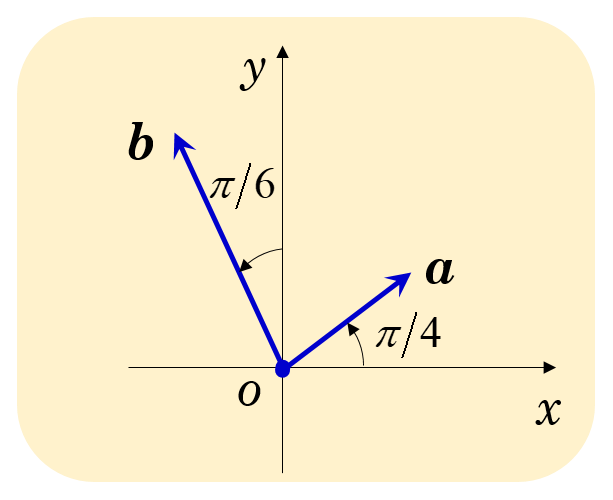
\includegraphics[width=0.3\linewidth]{fig1_1.eps} 
        \end{center}
        \caption{Vectors $\fat{a}$ and $\fat{b}$ in 2 dimensional space with an $xy$ Cartesian coordinate system.}
        \label{fig:fig1_1}
    \end{figure}

    {\small
    In terms of components, the given vectors are written as 
    \[
        \fat{a}= \left( \frac{1}{\sqrt{2}}, \, \frac{1}{\sqrt{2}}\right), 
        \fat{b}=2 \left( -\frac{1}{2}, \, \frac{\sqrt{3}}{2}\right).
    \]
    Hence,
    \[
        \fat{a}+\fat{b}=\left( \frac{1}{\sqrt{2}}-1, \frac{1}{\sqrt{2}}+\sqrt{3}\right),
    \]
    and 
    \[
        | \fat{a}+\fat{b}| = 
        \left\{
        \left( \frac{1}{\sqrt{2}}-1\right)^2 +
        \left( \frac{1}{\sqrt{2}}+\sqrt{3}\right)^2
        \right\}^{1/2}
        =
        \frac{\sqrt{11-2\sqrt{2}+4\sqrt{3}}}{2}.
    \]
    }
\item
    For vectors shown in Fig.\ref{fig:fig1_2}, prove that 
    \[
        \fat{a}+\fat{b}+\fat{c}=\fat{0}
    \]
    if $|\fat{a}|=|\fat{b}|=|\fat{c}|$.\\
    \begin{figure}[h]
    \begin{center}
        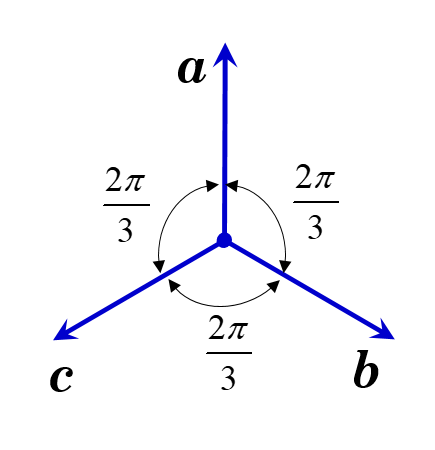
\includegraphics[width=0.3\linewidth]{fig1_2.eps} 
        \end{center}
        \caption{Vectors $\fat{a}, \fat{b}$ and $\fat{c}$ of equal magnitude.} 
        \label{fig:fig1_2}
    \end{figure}

    {\small
        By sliding vectors $\fat{b}$ and $\fat{c}$ as shown in Fig.\ref{fig:fig}, we can verify that the three vectors form a closed path. This means $\fat{a}+\fat{b}+\fat{c}=\fat{0}$. You may, otherwise, introduce a Cartesian coordinate, and show that the componentwise vector addtion results in zero vector. 
    }
    \begin{figure}[h]
        \begin{center}
        \includegraphics[width=0.25\linewidth]{fig1_2ans.eps} 
        \end{center}
        \caption{Slided replicas of vectors $\fat{b}$ and $\fat{c}$.} 
        \label{fig:fig1_2ans}
    \end{figure}
\item
    Suppose that a perfectly rigid bar AB is supported horizontally by a wall as shown in Fig.\ref{fig:fig1_3}. The bar is sufficiently long and is subjected to infinitely many vertical forces $\fat{f}_i (i=1,2,...)$ whose magnitude decreases monotonically as 
    \[
         \frac{ |\fat{f}_{i+1}| }{ |\fat{f}_i| } =\frac{9}{10} 
    \]
with $|\fat{f}_1|=F$. Determine the direction and magnitude of the total force acting acting to the bar.\\
\begin{figure}[h]
    \begin{center}
    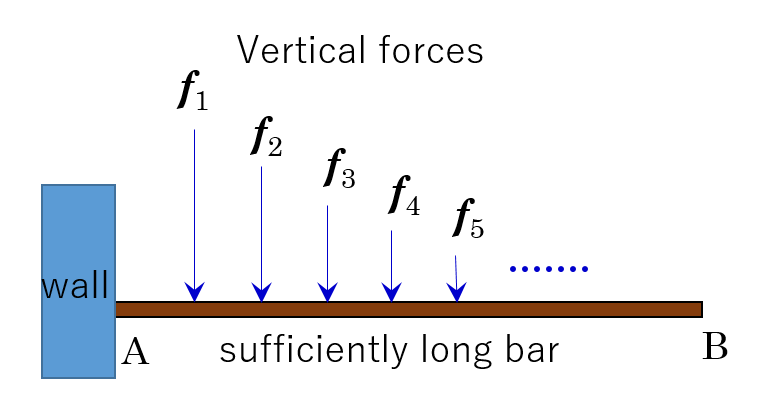
\includegraphics[width=0.5\linewidth]{fig1_3.eps} 
    \end{center}
    \caption{Infinitely many downward forces acting to a horizontally supported bar AB.}
    \label{fig:fig1_3}
\end{figure}

    {\small 
     In summing the force vectors, we only need to consider the vertical components since the horizontal components vanish altogether. If we write the vertical component of $\fat{f}_i$ as $f_{zi}$, and let 
        \[
            \gamma=\frac{|\fat{f}_{i+1}|}{|\fat{f}_i|}=\frac{9}{10},
        \]
        then we may write $f_{zi}$ as 
        \[
            f_{zi}=F\gamma^{i-1}, (i=1,2,\dots).
        \]
  Then, the first $n$ terms of $f_{zi}$ can be summed explicitly as  
        \[
            \sum_{i=1}^n f_{zi}=F\sum_{i=1}^n\gamma^{i-1}=F\frac{1-\gamma^n}{1-\gamma} >0
        \]
        where a positive vertical component means a donward force.
        Letting $n\rightarrow \infty$, we obtain the magnitude of the total force $\sum_{i=1}^\infty \fat{f}_i$ 
        as follows. 
        \[
            \left| \sum_{i=1}^\infty \fat{f}_i \right| =\frac{F}{1-\gamma}=10F
        \]
    }
\item
    Suppose that weight is hung from a ceiling by a string AB as shown in Fig.\ref{fig:fig1_4}-(a). Determine the magnitude of the horizontal force $F$ required to hold the weight as shown in Fig.\ref{fig:fig1_4}-(b).  Note that $m$ is mass and $g$ is the gravity constant. \\
    \begin{figure}[h]
    \begin{center}
    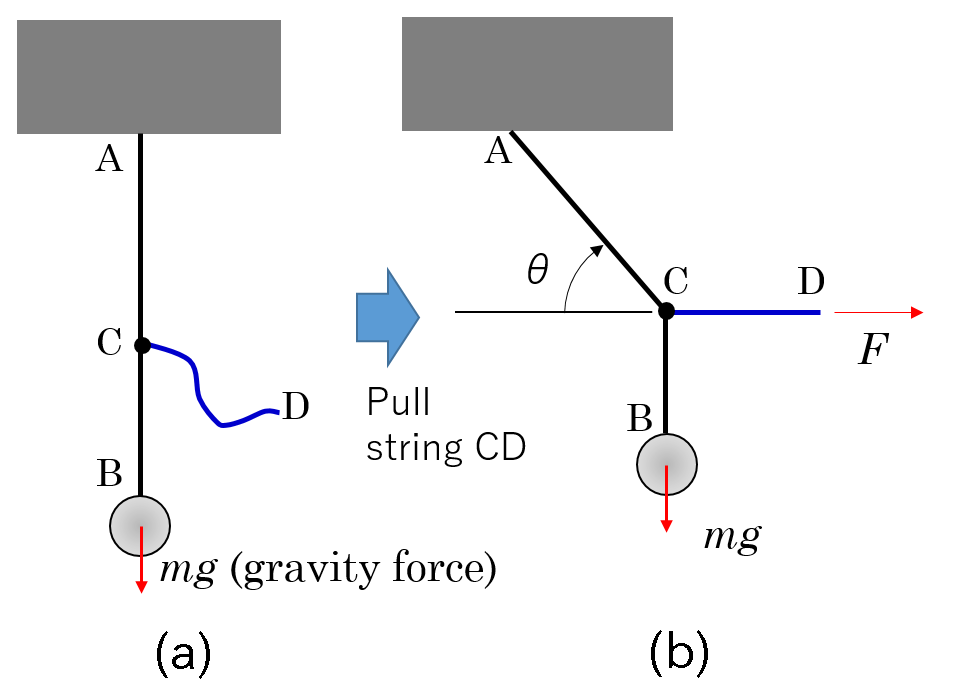
\includegraphics[width=0.6\linewidth]{fig1_4.eps} 
    \end{center}
    \caption{A weight of mass $m$ hung from a ceiling by a string AB.} 
    \label{fig:fig1_4}
    \end{figure}

    {\small
        Let the tensile forces acting in a string AC, DC and BC be 
        $\fat{T}_{AC}, \fat{T}_{DC}$ and $\fat{T}_{BC}$, respectively. 
        In the $xy$ Cartesian coordinate shown in Fig.*, the tensile force vectors are written as follows.
        \[
            \fat{T}_{AC}=|\fat{T}_{AC}|\left(-\cos\theta,\, -\sin\theta \right)
        \]
        \[
            \fat{T}_{DC}=\left(F,\,0 \right)
        \]
        \[
            \fat{T}_{BC}=\left(0,mg \right)
        \]
        At point C where the strings are joined, the sum of the tensile forces must vanish since the joint is in static equilibrium. Newton's second law requires 
        \begin{equation}
            \fat{T}_{AC}+ \fat{T}_{DC}+\fat{T}_{BC}=\fat{0}.
            \label{eqn:equivT}
        \end{equation}
In terms of vector components, eq.(\ref{eqn:equivT}) is written as
        \begin{equation}
            -|\fat{T}_{AC}|\cos\theta+F=0
            ,\ \ 
            -|\fat{T}_{AC}|\sin\theta+mg=0
            \label{eqn:}
        \end{equation}.
Thus we can conclude
        \begin{equation}
            |\fat{T}_{AC}|=\frac{mg}{\sin\theta}, \ \ 
            F=\frac{mg}{\tan\theta}. 
            \label{eqn:}
        \end{equation}
    }
\end{enumerate}
\section{Supplementary Problems}
\begin{enumerate}
\item
    Verify that the vector addition is associative, i.e., 
    \begin{equation}
        \fat{a}+(\fat{b}+\fat{c})= (\fat{a}+\fat{b})+\fat{c}
    \label{eqn:sprb1}
    \end{equation}
    using graphic representation of vectors. 
    (Draw arrows to represent $\fat{a},\fat{b}$ and $\fat{c}$. THen verify \ref{eqn:sprb1} holds.)
\item
    For unit vectors shown in Fig.\ref{fig:fig_5}, obtain $\fat{a}+\fat{b}+\fat{c}$.  
    \begin{figure}[h]
    \begin{center}
    \includegraphics[width=0.3\linewidth]{fig1_5.eps} 
    \end{center}
    \caption{Vectors $\fat{a}, \fat{b}$ and $\fat{c}$ in 2D space with an $xy$ Cartesian coordinate system.}
    \label{fig:fig1_5}
    \end{figure}
\item
    For given vector $\fat{c}$ of length $c$ shown in Fig.\ref{fig:fig1_6}, determine the lengths of vectors 
    $\fat{a}$ and $\fat{b}$ such that $\fat{a}+\fat{b}+\fat{c}=\fat{0}$.
    \begin{figure}[h]
    \begin{center}
    \includegraphics[width=0.3\linewidth]{fig1_6.eps} 
    \end{center}
        \caption{
            Vectors $\fat{a}$ and $\fat{b}$ of unknown lengths and a given vector $\fat{c}$ of $|\fat{c}|=c$.} 
    \label{fig:fig1_6}
    \end{figure}
\item
    Suppose that a sufficiently long bar is supported horizontally by a rigid wall as shown in Fig.\ref{fig:fig1_7}. The bar is subjected to infinitely many vertical forces $\fat{f}_1,\fat{f}_2,\dots $ of alternating directions. Determine the direction and the magnitude of the total force when the magnitude of the force decreases monotonically as 
    \begin{equation}
        \frac{| \fat{f}_{i+1}|}{|\fat{f}_i|}=\frac{2}{3}, \ \ (i=1,2,\dots)
        \label{eqn:}
    \end{equation}
 with $|\fat{f}_1|=F$.
    \begin{figure}[h]
    \begin{center}
    \includegraphics[width=0.45\linewidth]{fig1_7.eps} 
    \end{center}
    \caption{Infinitely many vertical forces of alternating direction acting to a horizontally supported bar AB.}
    \label{fig:fig1_7}
    \end{figure}
\end{enumerate}
\end{document}
\item
    Suppose that two weights of different mass ($m$ and $M$) are hung from a rigid ceiling as shown in Fig.\ref{fig:fig1_8}. Determine the ratio $M/m$ when the string BE is known to be tied horizontally and the weights and strings are in static equilibrium.
    \begin{figure}[h]
        \begin{center}
        \includegraphics[width=0.45\linewidth]{fig1_8.eps} 
        \end{center}
        \caption{Two weights of different mass hung from a ceiling by perfectly flexible strings} 
        \label{fig:fig1_8}
    \end{figure}
%%%%%%%%%%%%%%%%%%%%%%%%%%%%%%%%%%%%
